%%%%%%%%%%%%%%%%%%%%%%%%%%%%%%%%%%%%%%%%%%%%%%%%%%%%%%%%%%%%%%%%%%%%%%%%%%%%%%%%
%2345678901234567890123456789012345678901234567890123456789012345678901234567890
%        1         2         3         4         5         6         7         8
%
%\documentclass[letterpaper, 10 pt, conference]{ieeeconf}  % Comment this line out if you need a4paper
%
\documentclass[a4paper, 10pt, conference]{ieeeconf}      % Use this line for a4 paper
%
%\IEEEoverridecommandlockouts                              % This command is only needed if 
                                                          % you want to use the \thanks command
%
\overrideIEEEmargins                                      % Needed to meet printer requirements.
%
% See the \addtolength command later in the file to balance the column lengths
% on the last page of the document
%
\usepackage{graphicx} % for pdf, bitmapped graphics files
%\usepackage{hyperref}
%\hypersetup{colorlinks,urlcolor=blue,linkcolor=blue}
%
\usepackage{epstopdf}
%\usepackage{mathptmx} % assumes new font selection scheme installed
%\usepackage{times} % assumes new font selection scheme installed
\usepackage{amsmath} % assumes amsmath package installed
\usepackage{amssymb}  % assumes amsmath package installed

\usepackage{graphicx}
%\usepackage{subfig}
\usepackage{caption}
\usepackage{subcaption}
\usepackage{array}
\usepackage[space]{cite}

%\usepackage[hidelinks]{hyperref}
\usepackage[colorlinks, linkcolor = black, citecolor = black, filecolor = black, urlcolor = blue]{hyperref}


\usepackage{tikz}

\newcommand\encircle[1]{%
	\tikz[baseline=(X.base)] 
	\node (X) [draw, shape=circle, inner sep=0.5pt] {#1};}





%\DeclarePairedDelimiter\abs{\lvert}{\rvert}%
%\DeclarePairedDelimiter\norm{\lVert}{\rVert}%
\DeclareMathOperator*{\argmin}{argmin}
\DeclareMathOperator*{\argmax}{argmax}
\DeclareMathOperator*{\sgn}{sgn}
\newcommand{\specialcell}[2][c]{%
	\begin{tabular}[#1]{@{}c@{}}#2\end{tabular}}

\renewcommand{\citedash}{--}


\newcommand{\etal}{~\textit{et al.}}
%
\title{\bf {\LARGE Modern Myoelectric Intelligent Hand Prostheses} \\ 
{\normalsize H$^2$T-Seminar: Humanoid Robotics, WS 17/18}}
\author{Tobias Stocker, Pascal Weiner and Tamim Asfour \\ High Performance Humanoid Technologies \\ Institute for Anthropomatics and Robotics \\ Karlsruhe Institute of Technology \\
\url{http://www.humanoids.kit.edu}}


%
%
\begin{document}
\maketitle
\thispagestyle{empty}
\pagestyle{empty}
%
%%%%%%%%%%%%%%%%%%%%%%%%%%%%%%%%%%%%%%%%%%%%%%%%%%%%%%%%%%%%%%%%%%%%%%%%%%%%%%%%
\begin{abstract}
Myoelectric Hand Prostheses are an important research topic because these prostheses can improve the quality of life of amputees. The main goal in the design and development of prosthetic hands is to reach a high level of acceptance of the prostheses by potential users. Therefore the hand should look anthropomorphic and be rather lightweight while still enabling the user to do many different grasps with enough force and in short time without too much effort of the user. Another important factor is to keep the prosthetic hands as low-cost as possible to make them affordable for a wide audience of people.\\
In this paper different hand prostheses which were published in the last few years will be described and compared with each other with regard to various properties like weight, size and degrees of freedom as well as kinematics, mechanics, sensor systems and embedded systems. Additionally special features of the different prosthetic hands will be elaborated.
\end{abstract}

%%%%%%%%%%%%%%%%%%%%%%%%%%%%%%%%%%%%%%%%%%%%%%%%%%%%%%%%%%%%%%%%%%%%%%%%%%%%%%%%
\section{Introduction}

The goal of myoelectric hand prostheses is to make a normal life possible for amputees without any limitations. With current state-of-the-art technologies this isn't entirely possible but current developments at least aim to enable the users to do the most important activities of daily living (ADLs) and support them as good as they can. While currently available prosthetic hands take advantage of the latest technological advances, there are still a lot of open problems and many things to improve in regard to functionality, durability, cosmetic appearance and affordability~\cite{review}. Thus there is still ongoing interest into developing new myoelectric hand prosthesis and different research groups try to refine current designs and test new ideas.\\
There are a lot of desired properties a good prosthetic hand should fulfill but many of them contradict each other and therefore finding trade-offs is necessary, e.g. between affordability and functionality. The main goal when designing prostheses is to reach a high acceptance of possible users. One major aspect is comfortable wearing for long periods of time which requires low weight and small size. It is also important that the hand is easy to use and doesn't require too much concentration of the user. Additionally the prosthetic hand should be able to realize many different grasps with high finger forces and fast joint speeds to enable the user to hold a lot of different objects and use them for different tasks. Furthermore it should be robust and durable to bear with daily wearing and should be low-cost to be affordable for everyone who needs it, especially for people in developing countries.\\
In this paper different hand prostheses published in the last three years by research groups are considered. The properties and used technologies of each hand are elaborated on and the hands are compared with each other with regard to their properties, special features and focus of the design. The presented hands are the Tact~\cite{tact}, the hand of Bennett et al.~\cite{bennett}, the hand of Zhang et al.~\cite{zhang}, the MyHand~\cite{myhand}, the AstoHand v.1~\cite{astohand}, the X-Hand~\cite{xhand}, the Six-DOF-Hand~\cite{6dofhand}, the Bionic Hand~\cite{bionichand}, the SoftHand Pro-D~\cite{softhand}, the UOMPro~\cite{uompro} and the MORA Hap-2~\cite{morahap2}. Since the currently commercially available hands are for the most part still the same hands mentioned in\cite{review} (Vincent Hand~\cite{vincent}, iLimb~\cite{ilimb}, Bebionic~\cite{bebionic} and Michelangelo~\cite{michelangelo}) only research hands will be considered in this paper.
 

\section{Overview}

\subsection{Tact}

The Tact~\cite{tact} hand is an open-source myoelectric prosthetic hand developed by the Department of Mechanical Science \& Engineering and the Department of Aerospace Engineering of the University of Illinois with the goal to design a hand which is affordable for people in developing countries. Therefore tradeoffs between cost, performance, duration, efficiency and manufacturability were evaluated to find a possible way to make the hand low-cost while still maintaining performance similar to commercial prosthetic hand. They use lower-cost motors and don't use a complex tendon-driven design as joint actuation method but rather a simplified method consisting of a DC motor and a spool. As joint coupling method a four-bar linkage is chosen to produce consistent movement and strong forces at the finger tips. The joints of the fingers can reach a rather high joint speed of 250 $^\circ$/s.

\begin{figure}[h]

	\centering
	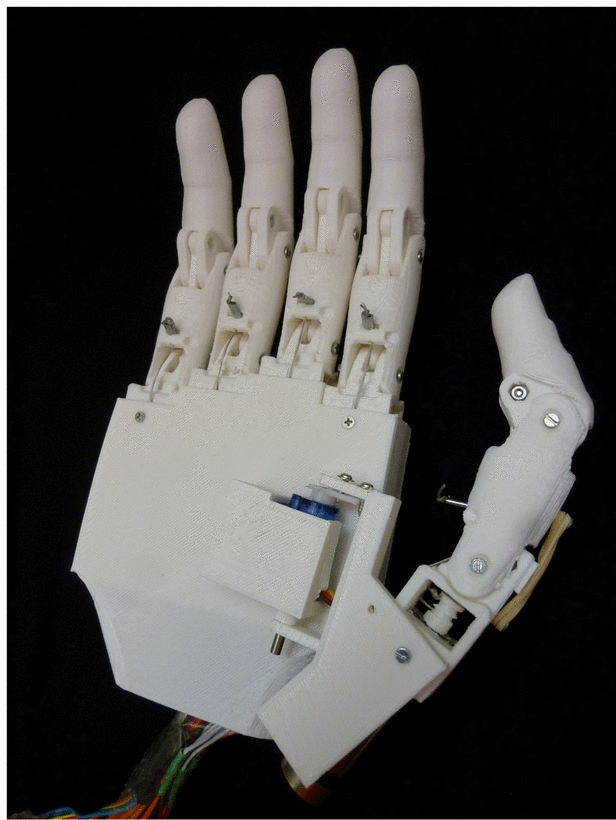
\includegraphics[scale=0.25]{images/Tact}
	
	\caption{The Tact}
\end{figure}

\subsection{Hand of Bennett et al.}

The hand of Bennett et al.~\cite{bennett} was developed by the Department of Mechanical Engineering of the Vanderbilt University. It incorporates four independent actuators in an unique configuration to provide precision grasps as well as whole-hand grasps. The thumb and the index finger which are responsible for precision grasps are both designed with three fully actuated joints to ensure good control during theses grasps. The first motor unit provides abduction/adduction of the thumb and the second motor unit provides flexion/extension of the thumb at the carpometacarpal (CMC) joint while the metacarpal phalangeal (MCP) and proximal interphalangeal (PIP) joints are fused. The third motor unit provides flexion/extension of the index finger at the MCP joint while the PIP and distal interphalangeal (DIP) joints are fused. The other three fingers which are responsible for stabilizing during whole-hand grasping are designed in an underactuated configuration where a single actuator controls all six joints to ensure good stability. The thumb and the index finger are actuated via bidirectional tendons while the other fingers are actuated via unidirectional tendons.\\
The hand mainly consists of a high-modulus material to form the load-bearing geometric and kinematic structure and a low-modulus structure to provide a softer cover to facilitate grasping of objects. The hand includes an embedded system consisting of a single, four-layer circuit board which is fully contained within the palm of the prosthetic hand. It accepts and executes motion and force commands from a high-level controller via a controller area network (CAN) serial interface and returns processed position and force information.

\begin{figure}[h]

	\centering
	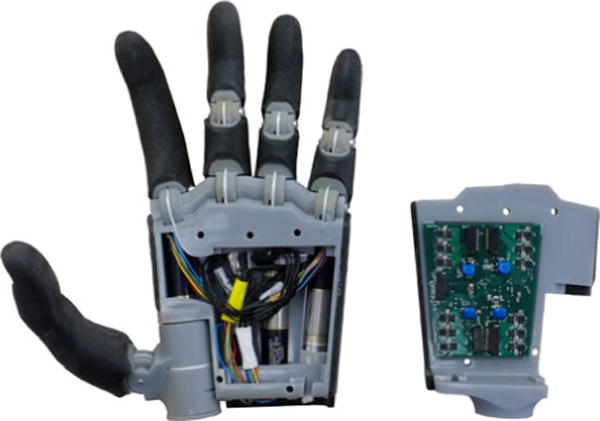
\includegraphics[scale=0.7]{images/Bennett}
	
	\caption{The Hand of Bennet et al.}
\end{figure}

\subsection{Hand of Zhang et al.}

The hand of Zhang et al.~\cite{zhang} was developed mainly by the Guangdong Provincial Key Laboratory of Robotics and Intelligent Systems in the Chinese Academy of Sciences and consists of five fingers and 15 joints, with each finger being actuated by one embedded DC motor. From their point of view this is the most balanced approach in terms of efficiency, response time and reliability. The design of the index/middle finger and of the ring/little finger are different from each other to make the motion of the fingers more natural, to make more grasp patters possible and to make them adaptive to the object shape. A four-bar linkage mechanism was chosen as actuation mode instead of a tendon driving mechanism because they came to the result that it has more stability and can reach higher grasping forces. A coupling link mechanism was selected over an underactuated mechanism for the design of the fingers except for the thumb. While the underactuated mechanism makes an adaptive grasping mode possible, it was found out to be too complex and too bulky for their prosthetic hand. Since the thumb plays an important role in most grasping operations they tried to enable the thumb to grasp along a cone surface, similar to the human hand. For this the metacarpal of the thumb is placed at 30$^\circ$ deflection to the base joint of the middle finger and with an initial abduction of 30$^\circ$ to the palm.\\
Dedicated torque and position sensors were developed for the prosthetic hand. They are used to guarantee control schemes such as impedance control in autonomous operations. The hand contains 18 proprioceptive and exteroceptive sensors: the base joints contain five Hall effect joint position sensors and five strain gauge joint torque sensors for measuring the grasping force of each finger, the palm contains five current sensors for the five DC motors and each motor in the thumb, index and middle finger contains three incremental encoders.\\
The mechanical parts, electronics and the motion control system are embedded in the hand. The motion control system consists of a small light weight motion control subsystem with high speed computation and several sensory subsystems. The motion control subsystem includes a DSP chip, an A/D converter to sample the sensor signals for torque and position, a CAN module to communicate with the mutual perception system and a serial communication module to connect the motion control system and a PC for debugging and operator training.\\
A sensory feedback system is used to help the amputees to control the force as they intend. The motion control system acquires and grades the force data and sends it to the man-machine interface. The man-machine interface generates constructive parameters based on a typical stimulation strategy and transmits them to the stimulator which produces concrete stimulus waveforms. The stimulator can be attached to the amputee's body and stimulus is then applied so he can feel the actual force exerted by the hand prosthesis.

\begin{figure}[h]

	\centering
	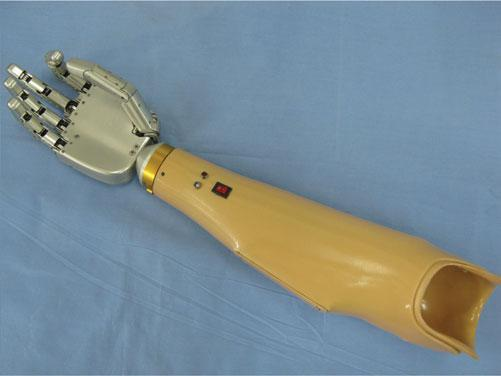
\includegraphics[scale=0.7]{images/Zhang}
	
	\caption{The Hand of Zhang et al.}
\end{figure}

\subsection{SSSA-MyHand}

The MyHand~\cite{myhand} was developed by the BioRobotics Institute of the SSSA and published in 2016. The goal was to design a dexterous lightweight hand prosthesis as an alternative to clinically available multi-grasp prostheses while using low-cost manufacturing processes and components wherever possible. To reduce complexity the hand carries three identical 8W brushless DC motors, one for the flexion/extension of the thumb, one for the abduction/addutcion of the thumb as well as for the flexion/extension of the index finger and one for the flexion/extension of the other three fingers. The functional components are held together by a thin plate surrounded by a 3D-printed metallic mainframe and plastic covers for protection.\\
The hand includes a special transmission mechanism which implements a semi-independent actuation of the abduction/adduction of the thumb and the flexion/extension of the index finger with a single actuator. This so called TISIT (Thumb-Index Semi-Independent Transmission) combines a Geneva drive and a four-bar mechanism. The input of the TISIT is connected to the drive wheel of the Geneva drive as well as to the four-bar mechanism. The output of the Geneva drive is used for the abduction/adduction of the thumb while the output of the four-bar mechanism is used for the flexion/extension of the index.\\
The prosthetic hand also contains a sensory system for automatic grasp control and makes a future integration of a sensory feedback system possible which returns a signal to the user via vibrations. The motors are controlled by the master microcontroller which also acquires the EMG singals and communicates with a high-level controller outside of the hand. The master microcontroller gains information about the actual speed and position of the motors from a slave microcontroller which samples this information through Hall-effect sensors in the actuators.\\
The force exerted at the fingertips is on average 31.4 N for the thumb, 11.7 N for the index finger and between 9.4 N and 14.6 for the other three fingers. The flexion/extension speed is 160 $^\circ$/s for the thumb and 170 $^\circ$/s for the other fingers, while the speed of the thumb while switching from the opposition to the reposition state can reach 250 $^\circ$/s. The time needed to complete a grasp starting from the rest position is 270 ms for a lateral grasp and 370 ms for a cylindrical grasp.

\begin{figure}[h]

	\centering
	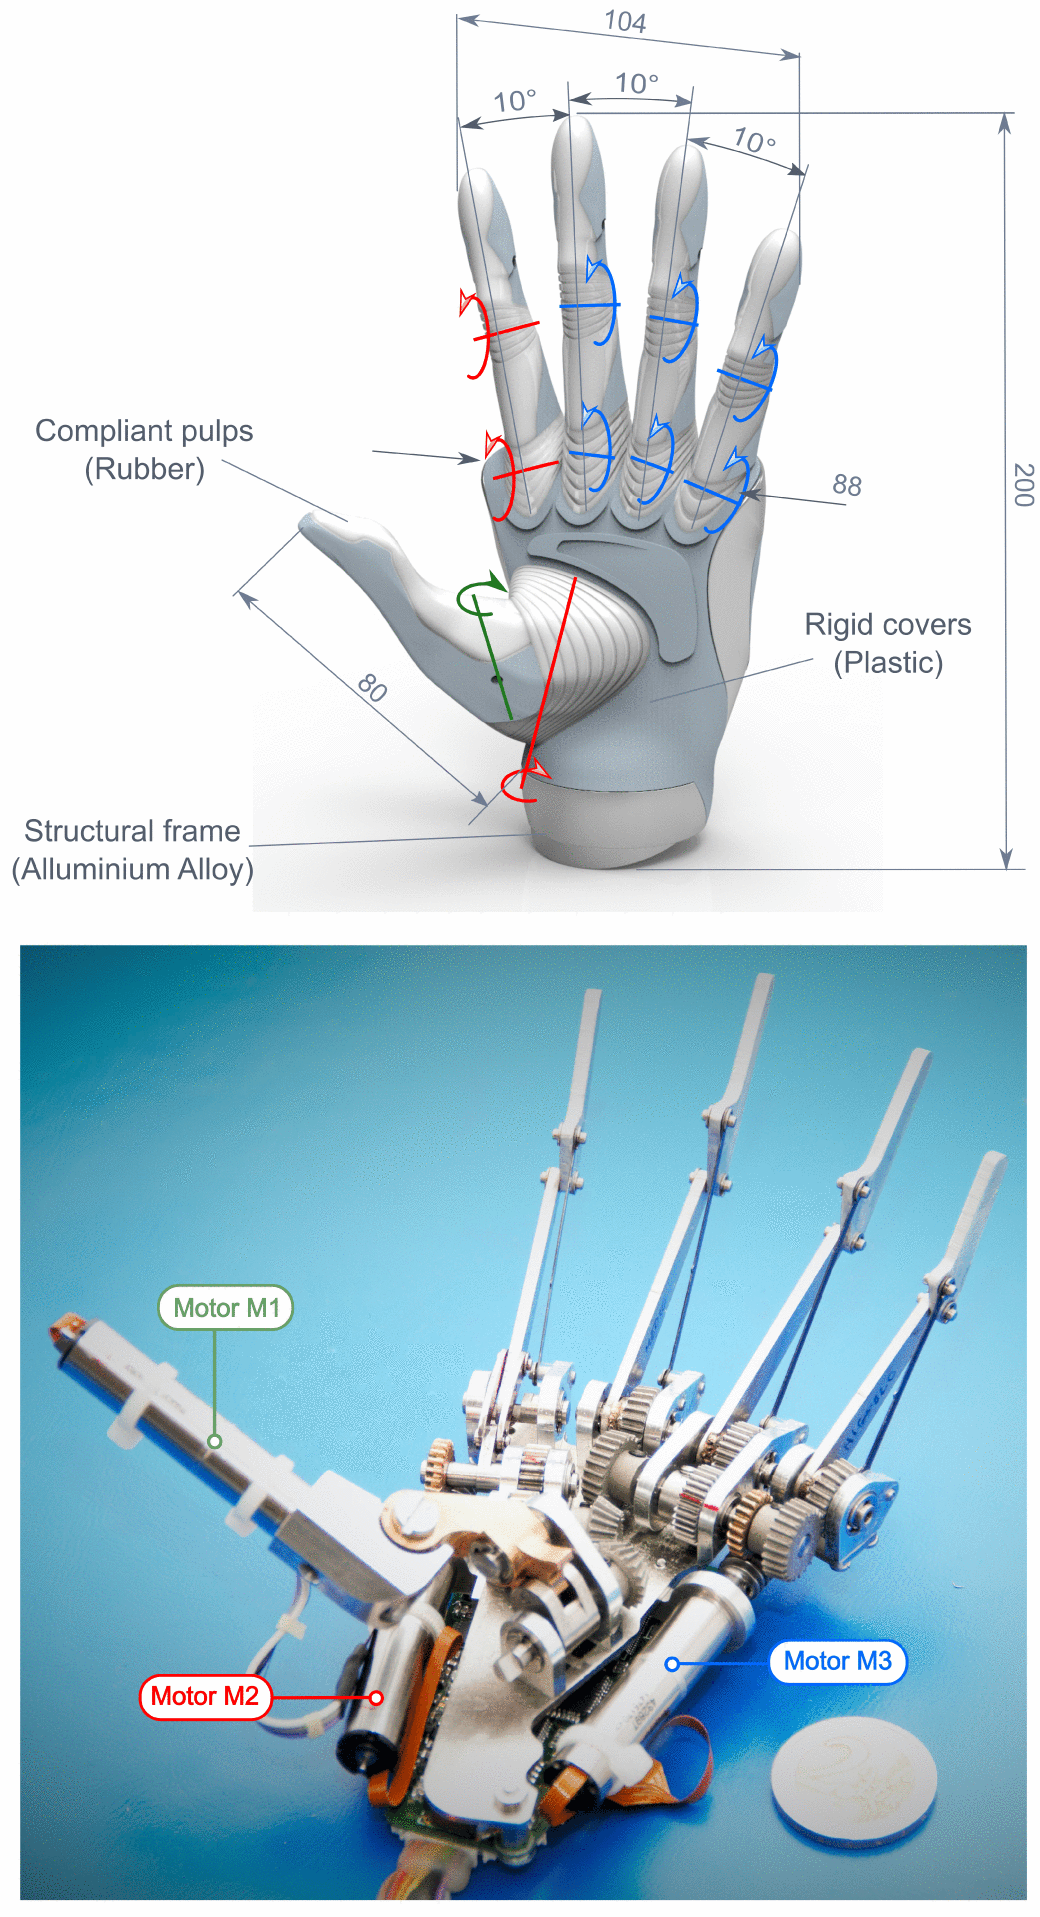
\includegraphics[scale=0.15]{images/MyHand}
	
	\caption{The MyHand}
\end{figure}


\subsection{AstoHand v.1}

The AstoHand v.1~\cite{astohand} was developed by the Department of Mechanical Engineering of the Diponegoro University. They focused on designing a low-cost anthropomorphic prosthetic hand which uses DC micro metal gear motors and 3D-printed material to make it lightweight. The developed hand has two joints per finger and each finger is powered by one motor. This configuration was chosen because it is sufficient for the most important activities of daily living while reducing the complexity of the mechanical design and manufacturing costs. For the movement of the fingers the motors are connected to the joints via a tendon-spring mechanism. The five DC motors are placed in the palm, an Arduino Nano microcontroller and driver motor are placed in the back cover and two batteries, with voltage of 3.7 V and capacity of 2425 mAh, are placed in the socket of the hand. The control algorithm of the hand is developed in Simulink and the digital input is used to read the tactile switch state for selecting one of the seven grip patterns.

\subsection{X-Hand}

The X-Hand~\cite{xhand} is an anthropomorphic prosthetic hand with size similar to the human hand designed by the Institute of Rehabilitation and Medical Robotics at the Huazhong University of Science and Technology. The goal was to design a hand prosthesis which fulfills the following three important features: Anthropomorphic grasp functions to cover the activities of daily living, few actuators to reduce complexity and easy control, and a compact structure with integrated hardware for a flexible installation and convenient wearing for the user.\\
The thumb mechanism of the X-Hand is designed independently of the mechanism of the other fingers to enable the thumb to move independently during grasping like in the human hand. Two DC motors are used for the kinematic transmission system of the four fingers to generate anthropomorphic grasping movements and two DC motors are used for the movement of the thumb. The time needed to close the hand from open is 1.2 s. The grasping force measured during contact with a cylinder between thumb and index finger is 12.1 N.

\subsection{Six-DOF-Hand}

The Six-DOF-Hand~\cite{6dofhand} is a hand prosthesis developed by the Mechanical Engineering Department of the University of Colorado-Denver. One of the major goals of the project was to design a hand which is inexpensive and also open source. The hand is able to do any of the standard grasps (e.g. tip, palmar, lateral, cylindrical) as well as more complex tasks with independent finger movement. To keep the prosthetic hand low-cost a design with six actuators was chosen, which includes two motors for the thumb, for performing flexion/extension and rotation, and one motor each for the other fingers. The MCP and PIP joints are coupled through a belt system, while the DIP joint is fixed. The actuators include encoders to allow motor position feedback and the fingershells of the hand contain internal space to leave the possibility of embedding force sensing elements and flex-sensors open.

\subsection{Bionic Hand}

The Bionic Hand~\cite{bionichand} is a hybrid actuated prosthetic hand with a total of 24 joints developed by the Department of Biomedical Engineering of the Bogazici University and the Department of Mechatronic Engineering of the Marmara University. The goal of the design of the prosthesis was to replicate the human hand as accurately as possible with all its joints and connections. Neural Networks are used to classify the EMG signals as well as to control the actuators which include brushless DC motors and Shape Memory Alloy (SMA) actuators. The two types of actuators are used to imitate extrinsic and intrinsic muscles and to emulate the antagonistic contraction. Overall there are 13 motors placed in the forearm, four motor pairs for the flexion and extension of the four fingers, two motors for the flexion-extension and abduction-adduction of the wrist and three motors for controlling the thumb. The SMA actuators are placed on the sides of the metacarpals and are used for the abduction-adduction of the fingers. While they are rather slow and not strong in comparison to DC motors they are good to imitate the relatively weak intrinsic muscles because of their low weight and small size. But they also produce small amounts of linear displacement and heat management is needed~\cite{bundhoo}.


\subsection{SoftHand Pro-D}

The SoftHand Pro-D~\cite{softhand} is a prosthetic hand developed by the University of Pisa and the Instituto Italiano di Tecnologia whose design evolves from the Pisa/IIT SoftHand~\cite{pisahand}. The hand is highly underactuated by having 19 joints and only one single actuator. The hand consists of passive damping components and the desired motion is accomplished with the help of dynamic synergies. It can move in two different synergistic directions of motion to perform pinch grasps as well as power grasps. The proposed approach tries to exploit the frequency content of the EMG signals in an innovative and natural way, that means the speed of the muscle contraction is associated with the speed of the synergy. A low frequency in the EMG-signal leads to a low closing speed of the hand. The smaller fingers close a bit faster than the index finger whereby objects can be grasped between index finger and thumb with a precision grasp. A high frequency of the EMG-signal leads to a fast closing speed of the hand which can be used for power grasps. The single DC motor is located in the dorsal side of the palm and integrated in a support structure. The damping element lies parallel to the motor and is connected with a compression spring. Only the thumb is directly connected to the damper through a tendon.


\subsection{UOMPro}

The UOMPro~\cite{uompro} is an prosthetic hand developed by the Department of Mechanical Engineering of the University of Moratuwa. The designed hand has affordable costs and consists of six DOFs including flexion/extension for all five fingers and abduction/adduction of the thumb. Each finger of the hand consists of two joints, one proximal similar to the human MCP and one distal similar to both the human PIP and DIP. The DC geared micro motor in each finger can provide a torque of ~0.31 Nm which is further increased for the proximal joint by a worm and wheel gear system. The fingers are designed with a fixed relationships between the joint motions realized by a form of a four-bar linkage. The flexion/extension motion for the thumb is achieved by a motor on the thumb base also using a four-bar mechanism and the adduction/abduction is achieved by a motor located under the thumb base. The electronic components which are responsible for the low-level controlling are placed inside the hand and a serial communication interface is provided to enable communication to a high-level controller which sends either individual finger positions or hand grip pattern commands.

\subsection{MORA Hap-2}

The MORA Hap-2~\cite{morahap2} is a prosthetic hand with self-adaptive fingers developed by the Department of Mechanical Engineering of the University of Moratuwa. The transmission system and the actuators are all placed within a single unit. The prosthetic hand is capable of generating five different grasping patterns (cylindrical grasp, hook grasp, lateral pinch, tip pinch and palmar pinch). All fingers except for the thumb have the same mechanism consisting of two four-bar linkages connected at the PIP joint. Three torsion springs are attached at the joints of the fingers to limit joint motion of the four-bar mechanism and to help carry out the underactuation. The structure of the thumb is similar to the proximal and middle phalange of the normal finger mechanism. The thumb mechanism consists of a single four-bar linkage and two torsional springs and can generate flexion/extension and adduction/abduction with two separate motors. The finger mechanism of the prosthetic hand includes the ability of self-adaption to provide robust grasps for different objects. When the proximal phalange is in contact with the object during the grasping process, the PIP joint continues to rotate compressing the torsion spring inside the first four-bar linkage until the middle phalange gets in contact with the object. Then the DIP joint continues to rotate until the distal phalange gets in contact with the object and the object is grasped properly. This means the joints of the fingers are capable of adopting their angles passively according to the geometry of the object to ensure a robust grasp.



%\newpage~\newpage

\begin{table*}

\begin{tabular}{p{2.4cm}|p{1.8cm}|p{0.8cm}|p{1cm}|p{2.6cm}|p{1.2cm}|p{1.2cm}|p{1.2cm}|p{1.2cm}}

Name & Developer & Year & Mass(g) & Size (mm) length x width x thickness & Number of fingers & Number of joints & Joints per finger & Number of actuators\\
\hline
Tact~\cite{tact} & Slade et al. & 2015 & 350 & 200 x 98 x 27\newline 85th x 99th x 50th(f) & 5 & 11 & 3/2 & 6\\
\hline
-~\cite{bennett} & Bennett et al. & 2015 & 546 & 200 x 89 x -\newline 85th x 35th x - & 5 & 12 & 3/3/2 & 4\\
\hline
-~\cite{zhang} & Zhang et al. & 2015 & 420 & 159 x 79 x 21\newline 5th(f) x 50th(f) x 1st(f) & 5 & 15 & 3/3 & 5\\
\hline
MyHand~\cite{myhand} & SSSA & 2016 & 478 & 200 x 84 x 56\newline 85th x 50th x - & 5 & 10 & 2/2 & 3\\
\hline
AstoHand v.1~\cite{astohand} & Ariyanto et al. & 2016 & 261 & 180 x 85 x 50\newline 50th(f) x 50th x - & 5 & 10 & 2/2 & 5\\
\hline
X-Hand~\cite{xhand}& Xiong et al. & 2016 & - & human hand size & 5 & 16 & 4/3 & 4\\
\hline
Six-DOF-Hand~\cite{6dofhand} & Krausz et al. & 2016 & 584 & 202 x 99 x 61\newline 85th x 99th x - & 5 & 10 & 2/2 & 6\\
\hline
Bionic Hand~\cite{bionichand} & Atasoy et al. & 2016 & - & - & 5 & 24 & 3/4 & 13\\
\hline
SoftHand Pro-D~\cite{softhand} & Piazza et al. & 2016 & - & - & 5 & 19 & 3/4 & 1\\
\hline
UOMPro~\cite{uompro} & Nisal et al. & 2017 & 432 & 199 x 88 x -\newline 85th x 35th x - & 5 & 10 & 2/2 & 6\\
\hline
MORA Hap-2~\cite{morahap2} & Gopura et al. & 2017 & 250 & 95(fingers) x 83 x 25\newline - x 50th x 5th(f) & 5 & 14 & 2/3 & 4\\


\end{tabular}

\caption{Table with developer, year of publication, physical properties and information about joints and motors.\newline The additional line in Size states which percentile of a male hand (or female if stated) the value corresponds to.\newline The joints per finger are subdivided into thumb/(index/)others.}
\label{table:table1}

\end{table*}

\vspace{10cm}

\begin{table*}[h]

\begin{tabular}{p{2.4cm}|p{2cm}|p{1.2cm}|p{2.1cm}|p{2cm}|p{1.5cm}|p{1.5cm}|p{1.2cm}}

Name / \newline Developer & Actuator type & Actuators integrated & Transmission system & Sensor system & Individual\newline Finger Force & Joint Speed & Closing Time\\
\hline
Tact & DC Motor & Yes & Four-bar linkage & - & 4.21 N & 249.8 $^\circ$/s & -\\
\hline
Bennet et al. & Brushless\newline DC Servomotor & Yes & Tendons & Hall effect / force & 30 N / 30 N / 7 N & - & -\\
\hline
Zhang et al. & DC Motor & Yes & Four-bar linkage & torque / angle / position & 10 N / 10 N / 4.3 N & 68-118 $^\circ$/s & 1 s\\
\hline
MyHand & Brushless\newline DC Motor & Yes & Four-bar linkage /\newline Geneva drive & Hall effect / motor position / speed & 31 N / 12 N & 160-250 $^\circ$/s & -\\
\hline
Asto Hand v.1 & DC Motor & Yes & Tendon-spring & - & - & - & -\\
\hline
X-Hand & DC Motor & Yes & Tendons & - & - & - & 1.2 s\\
\hline
Six-DOF-Hand & DC Motor & Yes & Gears / belts & motor position & 4.12 N & 128 $^\circ$/s & -\\
\hline
Bionic Hand & Brushless\newline DC Motor & No & Tendons & - & - & - & -\\
\hline
SoftHand Pro-D & DC Motor & Yes & Tendons & - & - & - & -\\
\hline
UOMPro & DC Micro Motor & Yes & Four-bar linkage & - & - & - & -\\
\hline
MORA Hap-2 & - & Yes & Four-bar linkage & - & - & - & -\\
 

\end{tabular}

\caption{Table with information about actuators, transmission and sensor systems and dynamic properties.\newline The individual finger forces are subdivided into thumb/(index/)others}

\end{table*}

\newpage~\newpage

\section{Comparison}

\subsection{Physical properties}

The average weight of a human hand is 400 g~\cite{humanbody}, which is around 0.5 $\%$ of the total body weight for women and around 0.6 $\%$ for men. Since hand prostheses are not connected through the skeleton like a human hand, users feel that prosthetic hands with this weight are already too heavy and not comfortable. Therefore one goal to increase acceptability of designed hand prostheses is to keep the weight as low as possible. The weight of the presented hands (see Table~\ref{table:table1}) varies from 250 g for the MORA Hap-2 to 584 g for the Six-DOF-Hand. Only for three out of the eight hands the weight is below the 400 g of a human hand, while the weight of the others is probably too high to wear comfortably for a longer duration. It is important to note that these weights are the values described by the respective research groups and may not always include all components of the complete hand.\\
Hand prosthesis naturally should have the average size of a human hand or even better the hand size of the actual patient. All presented hands are designed to have more or less the size of a human hand, while the length varies from 159 mm to 202 mm, the width from 79 mm to 99 mm and the thickness from 21 mm to 61 mm.

\subsection{Kinematics and Actuation}

All fingers of the eleven presented prosthetic hands have between two and four joints. There are many different combinations of joints. See~\ref{table:table1} for the exact distribution of the joints in the different hands.\\
Most of the hands have between four and six actuators, which means one or two actuators for the thumb and either one actuator for each other finger or one actuator for the index and one actuator for the other three fingers combined. The two hands with less actuators are on the one hand the MyHand with one motor for the thumb, one motor for thumb and index finger combined and one motor for the last three fingers and on the other hand the strongly underactuated SoftHand Pro-D which only uses one single motor for all five fingers. The only hand with more than six actuators as well as actuators located outside of the hand is the Bionic Hand with 13 actuators, three for the thumb, four pairs for the other fingers and two for the wrist.\\
As transmission system six hands use tendons, while the MyHand uses a combination of four-bar linkage and Geneva drives, the Six-DOF-hand uses gears and belts and the hand of Zhang et al., the UOMPro and MORA Hap-2 use four-bar linkage.

\subsection{Grasping and dynamics}

The goal of all developed prosthetic hands is to have sufficient grasping patterns for various activities of daily living (ADLs). All presented hands are capable of most of the known grasping patterns including power grasps, precision grasps, lateral grasps and hook grasp except for the SoftHand Pro-D. But even this prosthetic hand with only one single actuator can move along two different synergistic directions of motion to perform either precision or power grasps.\\
For some of the prosthetic hands experiments were performed to obtain the maximal forces and joint speeds the hands can reach. The individual fingers of the Six-DOF-Hand and the Tact and the two small fingers of the hand of Zhang et al. can reach a force of about 4.2 N, while the other fingers of the hand of Zhang et al. and the normal fingers of the MyHand can reach a force of 10-12 N. The thumb of the MyHand and the thumb and index finger of the hand by Bennet et al. can reach a force of up to 31 N. Only for the X-Hand a total grasping force, which is the sum of all contact forces, is given and amounts to 12.1 N.\\
While the fingers of the human hand can reach a joint speed of up to 2290 $^\circ$/s during flexion the joint speed for everyday movements lies only between 172 and 200 $\circ$/s~\cite{weir}. Therefore this speed should be enough for activities of daily living. The joints of the MyHand, of the Six-DOF-Hand and of the hand of Zhang et al. can reach a speed of 120-160 $^\circ$/s. The base joint of the thumb of the MyHand and the joints of the Tact can reach a speed of 250 $^\circ$/s. The time needed to fully close the hand from open is 1.2 s for the X-Hand and 1 s for the hand of Zhang et al.

\subsection{Sensory systems}

The only hand with integrated sensors besides motor encoders is the hand of Zhang et al. which is equipped with 18 proprioceptive and exteroceptive sensors developed for the prosthetic hand. The hand of Bennett et al., the SSSA-MyHand, the Six-DOF-Hand and the UOMPro use motor encoder signals and Hall-effect sensors in the actuators to get force, speed and motor position feedback. The later three are also designed for future integration of touch sensors in the fingertips. The SSSA-MyHand has five lines used as digital input for integration of touch sensors and the Six-DOF-Hand has internal cavity in the finger shells to embed force sensing elements inside.\\
The SSSA-MyHand is the only prosthesis which considers sensory feedback to the user. It has output lines for future connection with a vibrotactile sensory feedback interface to transmit feedback as vibration to the user.

\subsection{Embedded systems}

An embedded system is specified for the hand of Bennett et al., the hand of Zhang et al., the SSSA-MyHand, the AstoHand v.1 and for the UOMPro. The embedded systems always consist of a low-level controller which receives motor position or grip pattern commands from a high-level controller and are responsible for controlling the motors and receiving sensor feedback from them. The high-level controllers are located outside of the hands and generate the motor position or grip pattern commands for the low-level controllers. For the hand of Bennett et al. it also processes the sensor feedback it receives from the low-level controller. In the SSSA-MyHand the sensor feedback is directly processed in the low-level controller. The low-level controller is divided into a master and a slave. While the master is responsible for communicating with the outside and controlling the motors the slave receives the sensor feedback and passes it to the master.


\section{Conclusion}

When designing myoelectric hand prostheses it is always necessary to find appropriate trade-offs between functionality, comfort and affordability. There are different research groups which develop prosthetic hands and try to optimize the design and find new approaches to increase the quality. Many research groups set their focus on one unique new feature while ignoring other important properties a prosthetic hand should fulfill. This helps to get recognition for new interesting approaches and may help other groups with their deign in the future but many hands developed in research are not suited for commercial distribution because they lack attributes which are important for high acceptance, e.g. they are too heavy or the actuation is too complex. The main goal in the last years was to develop preferably low-cost prostheses to make them affordable for a lot of people. Many research groups tried to find a good middle ground between high functionality and low costs and therefore the focus was not to incorporate novel intelligent functions.\\
Only the hand of Zhang et al. contains additional sensors in the joints outside of the actuators to get additional feedback. For five of the eleven hands an embedded system is specified. The embedded systems always consist of a low-level controller which receives motor position or grasp pattern commands from a high-level controller outside of the hand. The low-level controller is also responsible for controlling the actuators as well as to accept sensor feedback of the actuators.

\newpage

\bibliographystyle{./IEEEtran}
%\nocite{*}
\bibliography{./Ausarbeitung}
%
\end{document}
%